\documentclass{beamer}
\usepackage{listings}
\lstset{
%language=C,
frame=single, 
breaklines=true,
columns=fullflexible
}
\usepackage{subcaption}
\usepackage{setspace}
\usepackage{url}
\usepackage{tikz}
\usepackage{tkz-euclide} % loads  TikZ and tkz-base
%\usetkzobj{all}
\usepackage[utf8]{inputenc}
\usepackage{longtable}
\usetikzlibrary{calc,math}
\usepackage{float}
\newcommand\norm[1]{\left\lVert#1\right\rVert}
\renewcommand{\vec}[1]{\mathbf{#1}}
\usepackage[export]{adjustbox}
\usepackage[utf8]{inputenc}
\usepackage{amsmath}
\usetheme{Boadilla}
\newcommand\mytextbullet{\leavevmode%
\usebeamertemplate{itemize item}\hspace{.5em}}

\bibliographystyle{IEEEtran}

\usepackage{color}

\title{A Calculation of Cricket Ball Trajectories}
\author{B603 Research Team}
\institute{Indian Institute of Technology, Hyderabad.}
\date{\today}
\begin{document}


\begin{frame}
\titlepage
\end{frame}
\section{Introduction}
\begin{frame}
\frametitle{Introduction}
This article shows:\\
\begin{columns}
\column{1\textwidth}
  \begin{itemize}
  \item Constant force coefficient in sub-critical and super-critical Reynold number region.
  \item The transition between this two region with variable gradient.
  \item Approximate analysis of the trajectory equation which results very simple forms of trajectories.
  \item From the approximate analysis, the governing parameters are also observed.
  \item The effect of "No wind" and "Cross wind" on the trajectories of the cricket balls.
  \end{itemize}
\end{columns}

\end{frame}


\section{Literature Survey}
\begin{frame}
\frametitle{Literature Survey}
\begin{columns}
\column{1\textwidth}
  \begin{itemize}
  \item In [1-3], the authors have shown various forces on stationary balls with/without spin in wind tunnels of different types. So, \textbf{drag} and \textbf{side} forces are determined.
  \item In [4], some major simplifications are done in trajectory measurement. The trajectories of balls are studied in presence of different aerodynamic force profile.
  \item In [5], the trajectory of flying debris during extreme windstrom is calculated.
  
  \end{itemize}
\end{columns}

\end{frame}


\section{Trajectory Equation}
\begin{frame}
\frametitle{Trajectory Equation}

\begin{columns}
\column{0.5\textwidth}
  \begin{itemize}
  \item The trajectory equation is derived from [5], where the author sets an equation for both compact debris and sheet debris.
  \item For cricket balls, compact debris equation is used.
  
  
  \end{itemize}
%\end{columns}

\column{0.5\textwidth}
\begin{figure}[h!]
  \centering
  \begin{subfigure}[b]{0.6\linewidth}
    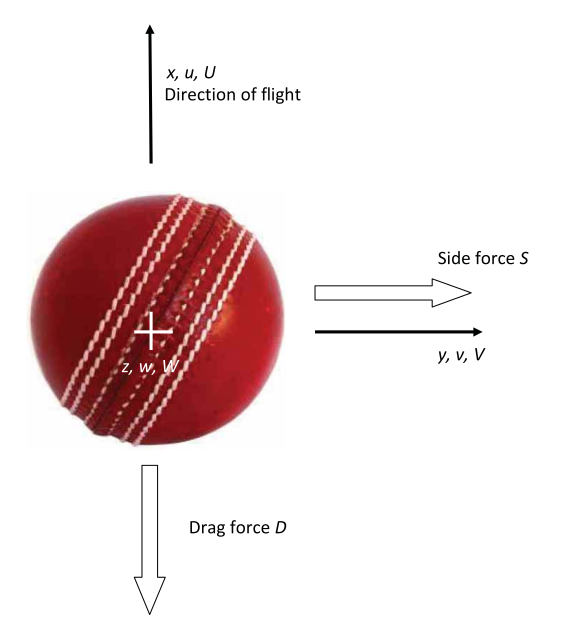
\includegraphics[width=\linewidth]{./figs/my_1.png}
%    \caption{Coffee.}
  \end{subfigure}

  \caption{Axis system, velocities, and forces}
  \label{fig:axis}
\end{figure}
\end{columns}

%\begin{columns}
%\column{.5\textwidth}
%  \begin{itemize}
%  \item First item.
%  \item Second item.
%  \end{itemize}
%\end{columns}

\end{frame}

\section{Trajectory Equation}
\begin{frame}
\frametitle{Trajectory Equation}
The basic trajectory equation for cricket balls:\\
\begin{align}
\frac{du}{dt}=-[(\vec{u}-\vec{U})^2+(\vec{v}-\vec{V})^2+(\vec{w}-\vec{W})^2]^{0.5}(\vec{u}-\vec{U})C_D T
%\label{equation: eq1}
\end{align}
\begin{align}
\frac{dv}{dt}=-[(\vec{u}-\vec{U})^2+(\vec{v}-\vec{V})^2+(\vec{w}-\vec{W})^2]^{0.5}[-(\vec{v}-\vec{V})C_D T+(\vec{u}-\vec{U})C_S T]
\end{align}
  
\begin{align}
\frac{dw}{dt}=-[(\vec{u}-\vec{U})^2+(\vec{v}-\vec{V})^2+(\vec{w}-\vec{W})^2]^{0.5}(\vec{w}-\vec{W})C_D T - 1
\end{align}


%  \doublespacing
%  
%  \item Where, $D$ = Drag force, $S$ = Side force, $\rho$= density of air, $Q$=total relative velocity of ball with respect to air, $T$ = Tachikawa number.
  
 


\end{frame}

\section{Trajectory Equation}
\begin{frame}
\frametitle{Trajectory Equation}
\begin{tabular} { | p {3 cm} | p {3 cm} | p {3 cm} | }
%\hline
%\multicolumn{3} { | c | }{Books}\\
\hline
Parameter symbol & Parameter name & Expression \\
\hline
$C_D$ & Drag Force Coeff. & $\frac{D}{0.5A \rho Q^2}$ \\
\hline
$C_S$ & Side Force Coeff. & $\frac{S}{0.5A \rho Q^2}$ \\
\hline
$T$ & Tachikawa no. & $\frac{\rho A q^2}{2mq}$ \\
\hline
$Re$ & Reynold no. & $\frac{q \rho d}{\mu}$ \\
\hline
\end{tabular}

\begin{tabular} { | p {3 cm} | p {4 cm} |  }
%\hline
%\multicolumn{3} { | c | }{Books}\\
\hline
Parameter symbol & Parameter name  \\
\hline
$D$ & Drag Force \\
\hline
$S$ & Side Force \\
\hline
$A$ & Ball cross-section area \\
\hline
$\rho$ & Density of air\\
\hline
$q$ & Initial speed of the ball\\
\hline
$m$ & Mass of the ball\\
\hline
\end{tabular}

\end{frame}

\section{Trajectory Equation}
\begin{frame}
\frametitle{Trajectory Equation}
\begin{tabular} { | p {3 cm} | p {4 cm} |  }
%\hline
%\multicolumn{3} { | c | }{Books}\\
\hline
Parameter symbol & Parameter name  \\
\hline
$d$ & Diameter of the ball \\
\hline
$\mu$ & Dynamic Viscosity of Air \\
\hline
$U$ & longitudinal wind speed \\
\hline
$V$ & lateral wind speed\\
\hline
$W$ & vertical wind speed\\
\hline
$u$ & longitudinal ball velocity\\
\hline
$v$ & lateral ball velocity\\
\hline
$w$ & vertical ball velocity\\
\hline
\end{tabular}
\end{frame}
\section{Reynolds number}
\begin{frame}{Reynolds number}
    \begin{itemize}
    \item 
    The drag and side force coefficients depends on the Reynolds number of the ball denoted by $Re$:
    \begin{align}
        Re = \frac{q\rho d}{\mu}
    \end{align}
    Where, 
    \begin{itemize}
        \item $q$ is the initial speed at which the ball is bowled,
        \item $\rho$ is the density of air, 
        \item $d$ is the diameter of the cricket ball and 
        \item $\mu$ is the dynamic viscosity of air.
    \end{itemize}
  \end{itemize}
\end{frame} 
\section{Significance of Reynolds number}
\begin{frame}{Significance of Reynolds number in cricket ball trajectory}
    \begin{itemize}
    \item 
    When the cricket ball travel through the air towards the batsman, the air flow around the ball can be \textbf{laminar} or \textbf{turbulent}.
    \item
    The \textbf{Reynolds} \textbf{number} is a parameter with determines the transition between from the laminar flow to turbulent flow. Thus, the Reynolds number plays a huge role in determining the drag and side force coefficients acting on the ball as the ball travels through air.
    \item
    For a cricket ball with diameter 7.2 $cm$ moving at 30 $m/s$ the Reynold’s number $Re$ is approximately 140,000. At a critical value of about 200,000 the laminar flow turns turbulent.
  \end{itemize}
\end{frame} 

\section{Significance of Reynolds number}
\begin{frame}{Laminar Flow}
    \begin{itemize}
    \item 
    In fluid dynamics, \textbf{laminar} flow is characterized by fluid particles following smooth paths in layers, with each layer moving smoothly past the adjacent layers with little or no mixing. 
    
    \item
    Similarly, when a cricket ball travels through air, the  air flows around the ball boundary is said to be \textbf{laminar} when the air flows on the either side of the ball follows a smooth path and does not mix with each other.   
    
    \item
    \textbf{Laminar} air flow occurs at lower ball velocity and when the balls is new with smooth surfaces.
    
  \end{itemize}
\begin{figure}[h!]
  \centering
  \begin{subfigure}[b]{0.4\linewidth}
    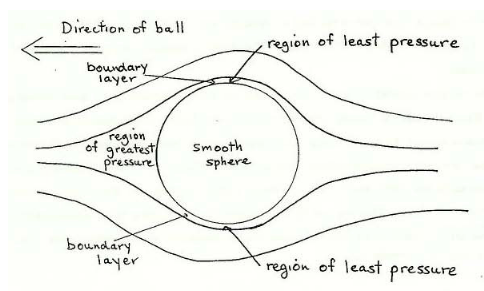
\includegraphics[width=\linewidth]{./figs/laminar.png}
    \caption{Laminar Flow}
  \end{subfigure}
\end{figure}
  
  
\end{frame} 
\section{Significance of Reynolds number}
\begin{frame}{Turbulent Flow}
    \begin{itemize}
    \item 
    In fluid dynamics, turbulence or \textbf{turbulent} flow is fluid motion characterized by chaotic changes in pressure and flow velocity. It is in contrast to a laminar flow, which occurs when a fluid flows in parallel layers, with no disruption between those layers.
    
    \item
    Similarly, when a cricket ball travels through air, the  air flows around the all boundary is said to be \textbf{turbulent} when the air flow around the ball  on the either side of the ball is chaotic and mixes with each other. 
    \item
     \textbf{Turbulent} air flow occurs at higher ball velocity and when the balls is old with rough surfaces.
  \end{itemize}
\begin{figure}[h!]
  \centering
  \begin{subfigure}[b]{0.4\linewidth}
    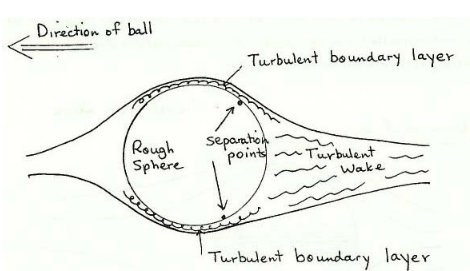
\includegraphics[width=\linewidth]{./figs/turbulant.png}
    \caption{Turbulent Flow}
  \end{subfigure}
  \caption{Different types of Flows}
  \label{fig:drag1}
\end{figure}
  
  
\end{frame} 

\section{Various cricket parameters which affect the Reynolds number of the ball.}
\begin{frame}{Various cricket parameters which affect the Reynolds number of the ball.}
    \begin{itemize}
    \item 
    The Reynolds number is directly proportional to \textbf{initial speed} of the ball bowled (denoted by $q$). A typical fast delivery is in the range of 85–95 mph (miles per hour), while most spin bowlers bowl at 45 to 55 mph.
     \item
    \textbf{Diameter} of the ball: The larger the ball's diameter, higher is the Reynolds number.
    \item 
    \textbf{Altitude} (from sea level): The density of air decreases with increasing altitude and thus affects the Reynolds number.
    \item
    \textbf{Humidity}: The addition of water vapor to air (making the air humid) reduces the density of the air (as molar mass of water is less than that of dry air), which in turn reduces the Reynolds number. 
    \item
    \textbf{Temperature}: High atmospheric temperature causes lower air density and  viscosity of air. Hence, temperature also affects the Reynolds number.
  \end{itemize}
\end{frame}

\section{Results of Past Experiments}
\begin{frame}
\frametitle{Results of Past Experiments}

\begin{figure}[h!]
  \centering
  \begin{subfigure}[b]{0.4\linewidth}
    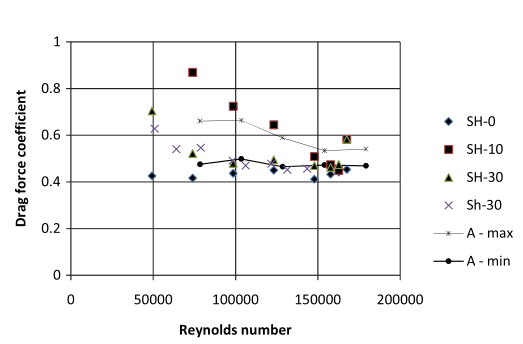
\includegraphics[width=\linewidth]{./figs/my_2.png}
    \caption{Smooth sphere/New Ball}
  \end{subfigure}
  \begin{subfigure}[b]{0.4\linewidth}
    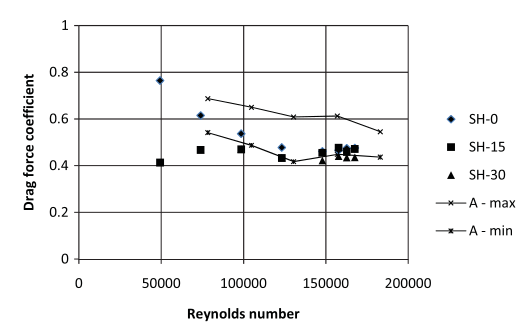
\includegraphics[width=\linewidth]{./figs/my_3.png}
    \caption{Rough Sphere/Old Ball}
  \end{subfigure}
  \caption{Compilation of cricket ball drag coefficient data}
  \label{fig:drag1}
\end{figure}
\end{frame}

\section{Results of Past Experiments}
\begin{frame}
\frametitle{Results of Past Experiments}

\begin{figure}[h!]
  \centering
  \begin{subfigure}[b]{0.5\linewidth}
    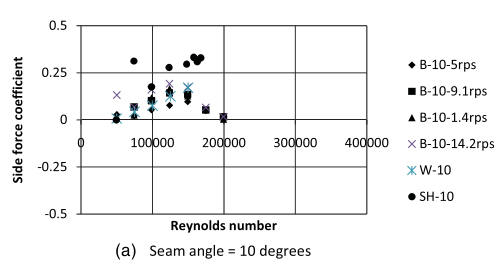
\includegraphics[width=\linewidth]{./figs/my_4.png}
%    \caption{Coffee.}
  \end{subfigure}
  \begin{subfigure}[b]{0.5\linewidth}
    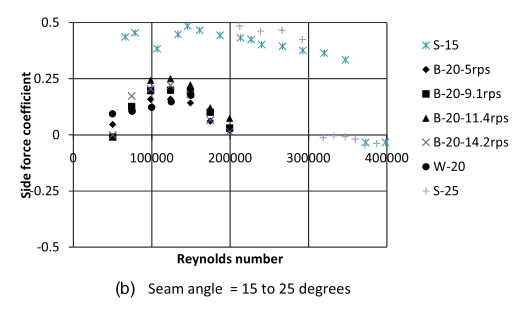
\includegraphics[width=\linewidth]{./figs/my_5.png}
%    \caption{More coffee.}
  \end{subfigure}
  \caption{Compilation of side force coefficient data for
smooth spheres/new balls.}
  \label{fig:side1}
\end{figure}
\end{frame}

\section{Results of Past Experiments}
\begin{frame}
\frametitle{Results of Past Experiments}

\begin{figure}[h!]
  \centering
  \begin{subfigure}[b]{0.5\linewidth}
    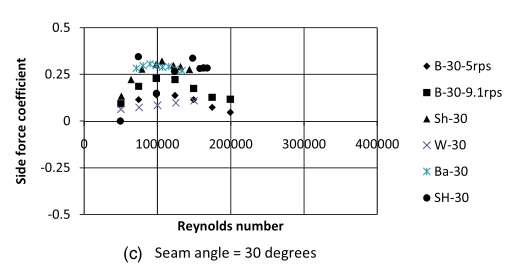
\includegraphics[width=\linewidth]{./figs/my_6.png}
    \caption{for
smooth spheres/new balls}
  \end{subfigure}
  \begin{subfigure}[b]{0.5\linewidth}
    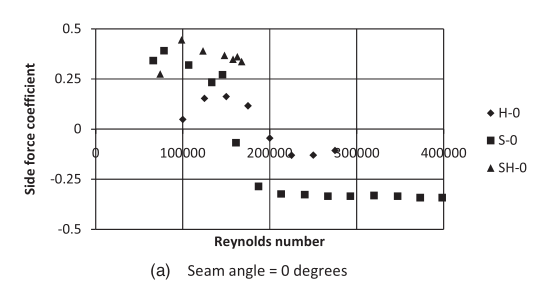
\includegraphics[width=\linewidth]{./figs/my_7.png}
    \caption{for semi-roughened spheres}
  \end{subfigure}
  \caption{side force coefficient data }
  \label{fig:side2}
\end{figure}
\end{frame}

\section{Results of Past Experiments}
\begin{frame}
\frametitle{Results of Past Experiments}
\begin{tabular} { | p {3 cm} | p {5 cm} |  }
%\hline
%\multicolumn{3} { | c | }{Books}\\
\hline
Symbol & Significance  \\
\hline
$SH-n$ & Experiments done by Sayer and Hill, n is the seam angle \\
\hline
$Sh-n$ & Experiments done by Sherwin, n is the seam angle \\
\hline
$B-n-m$ & Experiments done by Bentley, n is the seam angle, m is spin rate \\
\hline
$Ba-n$ & Experiments done by Bentley, n is the seam angle\\
\hline
$S-n$ & Experiments done by Sayer, n is the seam angle\\
\hline
$W-n$ & Experiments done by Ward, n is the seam angle\\
\hline
$H-n$ & Experiments done by Hunt, n is the seam angle\\
\hline
\end{tabular}
\end{frame}

\section{Results of Past Experiments}
\begin{frame}
\frametitle{Results of Past Experiments}

\begin{figure}[h!]
  \centering
  \begin{subfigure}[b]{0.5\linewidth}
    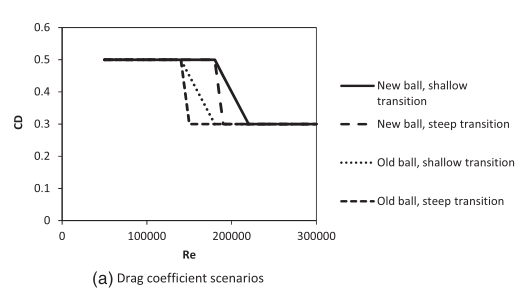
\includegraphics[width=\linewidth]{./figs/my_8.png}
%    \caption{Coffee.}
  \end{subfigure}
  \begin{subfigure}[b]{0.5\linewidth}
    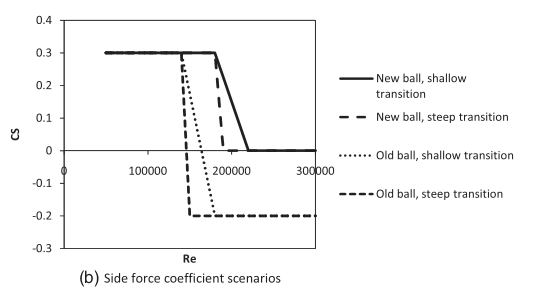
\includegraphics[width=\linewidth]{./figs/my_9.png}
%    \caption{More coffee.}
  \end{subfigure}
  \caption{Force coefficient scenarios for trajectory calculations}
  \label{fig:side3}
\end{figure}
\end{frame}

\section{Results of Past Experiments}
\begin{frame}
\frametitle{Observations}
From the plots \ref{side3}, it can be observed that:\\
\begin{itemize}
    \item 
    In sub-critical region the drag force coeffiecient is 0.5 for new ball as well as old ball.
     \item
    In super-critical region the drag force coeffiecient is 0.3 for new ball as well as old ball.
    \item 
    In sub-critical region the side force coeffiecient is 0.3 for new ball as well as old ball.
    \item
    In super-critical region the side force coeffiecient is 0 for new ball where as for old ball it is -2.5.
    \item
    These plots with different values of $C_D$ and $C_S$ are experimentally done, there  no particular expression of $C_D$ and $C_S$ are derived from the experimental data yet.
    
  \end{itemize}

\end{frame}


\section{Results of Past Experiments}
\begin{frame}
\frametitle{Steep and Shallow Transition}
\begin{tabular} { | p {3 cm} | p {5 cm} |  }
%\hline
%\multicolumn{3} { | c | }{Books}\\
\hline
Type of Transition & Range of Bowling speed   \\
\hline
Shallow Transition & 81 mile/hr to 100 mile/hr for new ball  \\
\hline
Steep Transition & 81 mile/hr to 86 mile/hr for new ball  \\
\hline
Shallow Transition & 63 mile/hr to 81 mile/hr for Old ball  \\
\hline
Steep Transition & 63 mile/hr to 68 mile/hr for Old ball  \\
\hline
\end{tabular}


\textbf{Significance}:\\
\begin{columns}
\column{1\textwidth}
  \begin{itemize}
  \item For both old and new ball, it is observed that in case of shallow transition the velocity of the ball is more than the velocity of the ball for steep transition at the end of the transition.
  
  \end{itemize}
\end{columns}



\end{frame}

\section{Approximate Solution}
\begin{frame}
\frametitle{Approximate Solution}

\begin{figure}[h!]
  \centering
  \begin{subfigure}[b]{0.4\linewidth}
    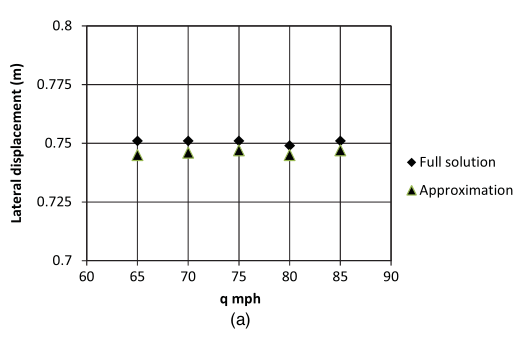
\includegraphics[width=\linewidth]{./figs/no_wind.png}
    \caption{No wind case}
  \end{subfigure}
  \begin{subfigure}[b]{0.4\linewidth}
    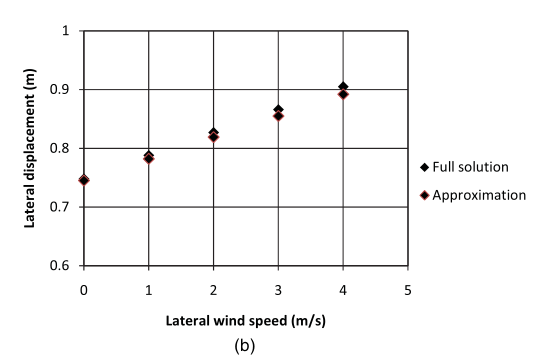
\includegraphics[width=\linewidth]{./figs/cross_wind.png}
    \caption{Cross wind case}
  \end{subfigure}
  \caption{Accuracy of approximate methods}
  \label{fig:Accuracy of approximate methods}
\end{figure}

\begin{columns}
\column{1\textwidth}
  \begin{itemize}
  \item \textbf{No wind case:} $\vec{U}=\vec{V}=\vec{W}=0$ and $C_D, C_S =$ constant,
  $ \vec{y}=\frac{C_S T}{2} \vec{x}^2$
  \item \textbf{Cross wind case:} $\vec{U}=\vec{W}=0$ and $\vec{V}\leq\vec{u}$ and 
 $ \vec{y}=\frac{(C_S + C_D \vec{V}) T}{2} \vec{x}^2$
  
  \end{itemize}
\end{columns}
\end{frame}


\section{Full Solution Trajectory Equation}
\begin{frame} 
\frametitle{Full Solution Trajectory Equation}

\begin{figure}[h!]
  \centering
  \begin{subfigure}[b]{0.5\linewidth}
    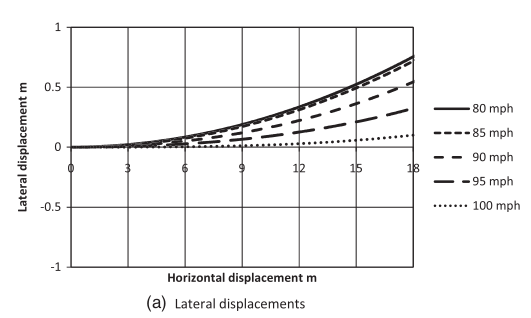
\includegraphics[width=\linewidth]{./figs/fs_1.png}
%    \caption{Coffee.}
  \end{subfigure}
  \begin{subfigure}[b]{0.5\linewidth}
    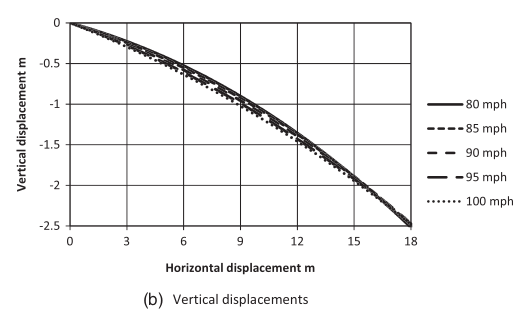
\includegraphics[width=\linewidth]{./figs/fs_2.png}
%    \caption{More coffee.}
  \end{subfigure}
  \caption{Trajectories for new ball/shallow transition sce-
nario.}
  \label{fig:fs12}
\end{figure}
\end{frame}

\section{Full Solution Trajectory Equation}
\begin{frame}
\frametitle{Full Solution Trajectory Equation}

\begin{figure}[h!]
  \centering
  \begin{subfigure}[b]{0.5\linewidth}
    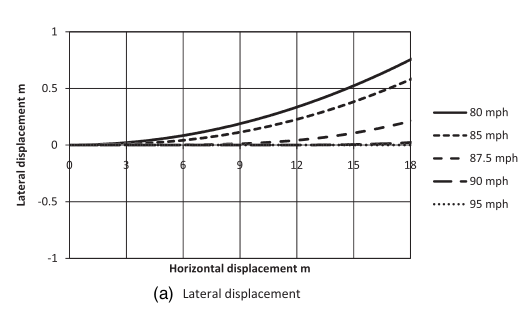
\includegraphics[width=\linewidth]{./figs/fs_3.png}
%    \caption{Coffee.}
  \end{subfigure}
  \begin{subfigure}[b]{0.5\linewidth}
    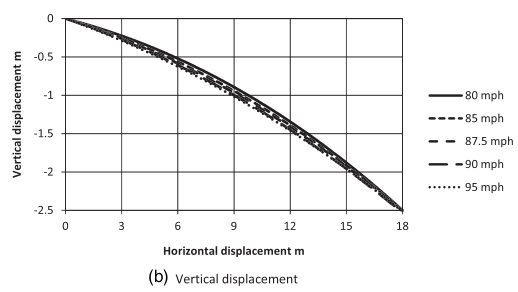
\includegraphics[width=\linewidth]{./figs/fs_4.png}
%    \caption{More coffee.}
  \end{subfigure}
  \caption{Trajectories for new ball/steep transition scenario.}
  \label{fig:fs34}
\end{figure}
\end{frame}

\section{Full Solution Trajectory Equation}
\begin{frame}
\frametitle{Full Solution Trajectory Equation}

\begin{figure}[h!]
  \centering
  \begin{subfigure}[b]{0.5\linewidth}
    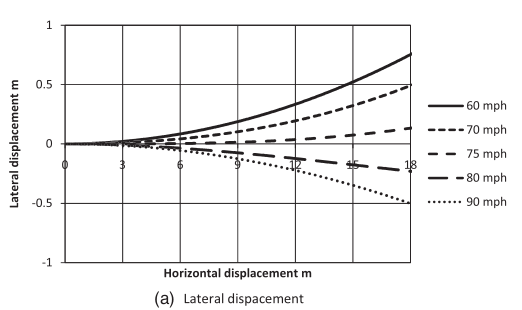
\includegraphics[width=\linewidth]{./figs/fs_5.png}
%    \caption{Coffee.}
  \end{subfigure}
  \begin{subfigure}[b]{0.5\linewidth}
    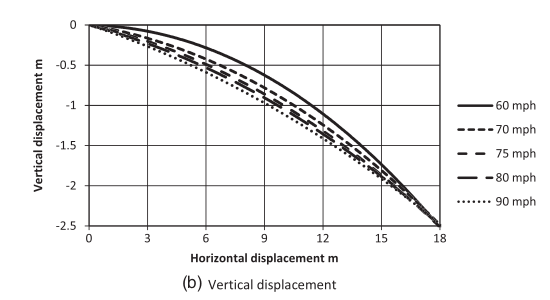
\includegraphics[width=\linewidth]{./figs/fs_6.png}
%    \caption{More coffee.}
  \end{subfigure}
  \caption{Trajectories for old ball/shallow transition sce-
nario.}
  \label{fig:fs56}
\end{figure}
\end{frame}

\section{Full Solution Trajectory Equation}
\begin{frame}
\frametitle{Full Solution Trajectory Equation}

\begin{figure}[h!]
  \centering
  \begin{subfigure}[b]{0.5\linewidth}
    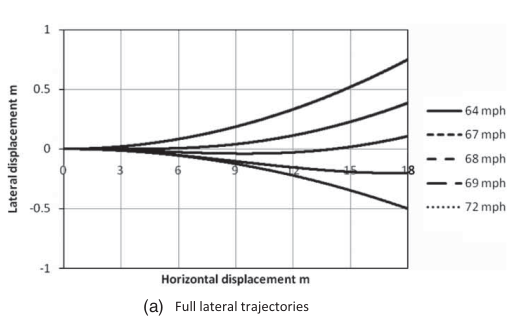
\includegraphics[width=\linewidth]{./figs/fs_9.png}
%    \caption{Coffee.}
  \end{subfigure}
  \begin{subfigure}[b]{0.5\linewidth}
    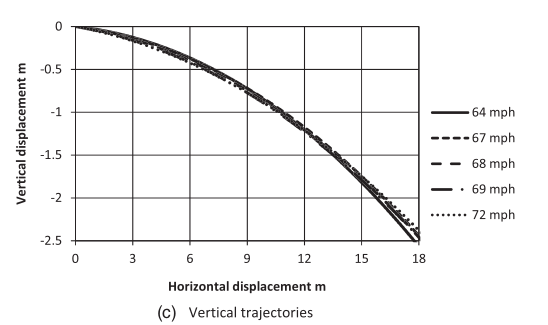
\includegraphics[width=\linewidth]{./figs/fs_8.png}
%    \caption{More coffee.}
  \end{subfigure}
  \caption{Trajectories for old ball/steep transition sce-
nario.}
  \label{fig:fs89}
\end{figure}
\end{frame}


\section{Conclusion}
\begin{frame}
\frametitle{Conclusion}
\begin{columns}
\column{1\textwidth}
  \begin{itemize}
  \item In trajectory equation, the main governing parameters are $C_D$, $C_S$ and $T$.
  \item The drag and side forces are reasonable constant in the sub and super crical Re number region.
  \item The supercritical values of the side force coefficient are in general zero for new balls, and less than zero for old balls.
  \item The approximate analysis of the trajectory equations shows that, for constant drag and side force coefficients, the trajectories take on a simple parabolic form.
  \item A full solution of the trajectory equations enables the trajectories to be calculated for all bowling speeds for different types of ball.
  \end{itemize}
\end{columns}

\end{frame}

%\begin{frame}
%
%\begin{columns}
%\column{.5\textwidth}
%  \begin{itemize}
%  \item First item.
%  \item Second item.
%  \item Third item.
%  \end{itemize}
%\setbeamertemplate{itemize items}[square]
%  \begin{itemize}
%  \item First item.
%  \item Second item.
%  \item Third item.
%  \end{itemize}
%\column{.5\textwidth}
%\setbeamertemplate{itemize items}[circle]
%  \begin{itemize}
%  \item First item.
%  \item Second item.
%  \item Third item.
%  \end{itemize}
%\setbeamertemplate{itemize items}[ball]
%  \begin{itemize}
%  \item First item.
%  \item Second item.
%  \item Third item.
%  \end{itemize}
%\end{columns}
%
%\end{frame}


\begin{frame}
\frametitle{Reference}
\begin{columns}
\column{1\textwidth}
  
\setbeamertemplate{itemize items}[square]
  \begin{itemize}
  \item [1]Mehta, R. D. Aerodynamics of sports balls. Annu. Rev.
Fluid Mech., 1985, 17, 151–189.
  \item [2]Mehta, R. D. Cricket ball aerodynamics: myth versus sci-
ence. In The engineering of sport – research, development
and innovation (Eds A. J. Subic and S. J. Haake), 2000,
pp. 153–167 (Blackwell Science, London).
  \item [3]Mehta, R. D. A review of cricket ball swing. Sports Eng.,
2005, 8, 181–192.
  \item [4]Bentley, K., Varty, P., Proudlove, M., and Mehta, R. D. An
experimental study of cricket ball swing. Imperial College
Aero Technical Note, 1982, pp. 82–106.
  \item [5] Baker, C. J. The debris flight equations. J. Wind Eng. Ind.
Aerodyn., 2007, 95(5), 329–353.
  \end{itemize}

\end{columns}

\end{frame}
\section{Back up}
\begin{frame}
\frametitle{Back up}
\begin{align}
\bar{x}= \frac{1}{C_D T}log(1+C_D T \bar{t})\\
\bar{y}= (\bar{t}-(\frac{1}{C_D T}log(1+C_D T \bar{t})))\frac{C_S}{C_D}\\
\bar{z}=\bar{t}\sin\alpha - \frac{\bar{t}^2}{2}
\end{align}
where
\begin{align}
\bar{t}= \frac{t g}{q}
\end{align}
$t$ is the time, $g$ is  acceleration due to gravity.

\end{frame}
\newpage
\bibliography{ref}

\end{document}

